\documentclass[handout]{beamer}
\usetheme{CambridgeUS}
\usecolortheme{beaver}
%note option
%\setbeameroption{show only notes}
%\usepackage{pgfpages}
%\setbeameroption{show notes on second screen}
% \setbeamertemplate{note page}[plain]
% \setbeamerfont{note page}{size=\scriptsize}
% \useoutertheme[subsection=false]{miniframes}
% end note option

\useinnertheme{circles}
\useoutertheme[subsection=false]{miniframes}
\setbeamertemplate{note page}[plain]
\setbeamertemplate{itemize items}[ball]
\setbeamertemplate{itemize subitem}[square]
\setbeamertemplate{itemize subsubitem}[triangle]
\setbeamertemplate{blocks}[rounded][shadow=true]
\setbeamertemplate{navigation symbols}{}
\setbeamertemplate{section in toc}[ball unnumbered]
\setbeamertemplate{subsection in toc}[triangle unnumbered]
\setbeamercolor{item}{fg=darkred}
\setbeamertemplate{headline}{}
\setbeamertemplate{itemize/enumerate body begin}{\small}
\setbeamertemplate{itemize/enumerate subbody begin}{\footnotesize}
\setbeamertemplate{footline}{\hfill\insertframenumber\vspace*{0.05in}\hspace*{0.05in}}

\usepackage{amsmath,amssymb}
\usepackage[T1]{fontenc}
\usepackage{url}
\usepackage{booktabs}
\usepackage{fancybox}
\usepackage[justification=centering,scriptsize]{caption}
\usepackage{colortbl}%for onslide uncover
\usepackage{cancel}
\usepackage{color}
\usepackage{multicol}
\colorlet{darkred}{red!50!black}
\colorlet{darkgreen}{green!50!black}
\newcommand{\bluealert}[1]{\textcolor{blue}{#1}}
\newcommand{\greenalert}[1]{\textcolor{darkgreen}{#1}}

\usepackage{tikz,tikz-3dplot}
%\usetikzlibrary{arrows,shapes}
\usetikzlibrary{
    shapes
  , shapes.misc
  , shadows
  , trees
  , arrows
  , arrows.meta
  , fit
  , calc
  , positioning
  , backgrounds
  , decorations
  , decorations.pathmorphing
  , decorations.text
  , decorations.pathreplacing
  , patterns
  , matrix
  , shadows
  , fit
  , chains
}

\usepackage{listings}
\lstset{basicstyle=\footnotesize\ttfamily,
  language=C,
  keywordstyle=\color{blue},
  ndkeywordstyle=\color{red},
  emphstyle=\color{red},
  commentstyle=\color{red},
  stringstyle=\color{dkgreen},
  backgroundcolor=\color{white},
  tabsize=2,
  showspaces=false,
  showstringspaces=false,
  breaklines,
  breakatwhitespace,
  mathescape,
  literate={"}{{\ttfamily"}}1
  {<-}{$\leftarrow$}2
  {!=}{$\neq$}1,
  columns=flexible,
}


\newenvironment<>{mblockvu}[1]{
  \setbeamercolor{block title}{bg=white,fg=black}
  \setbeamertemplate{blocks}[rounded][shadow=false]
  \setbeamertemplate{background canvas}[vertical shading][bottom=white,top=structure.fg!25]
  \setbeamertemplate{sidebar canvas left}[horizontal shading][left=white!40!black,right=black]
  \begin{block}#2{#1}}{\end{block}}


\newenvironment<>{mblock}[1]{
  \setbeamercolor{block title}{bg=white,fg=black}
  \begin{block}#2{#1}}{\end{block}}
\newenvironment<>{mredblock}[1]{
  \setbeamercolor{block title}{bg=red!30,fg=black}
  \begin{block}#2{#1}}{\end{block}}
\newenvironment<>{mblueblock}[1]{
  \setbeamercolor{block title}{bg=blue!30,fg=black}
  \begin{block}#2{#1}}{\end{block}}
\newenvironment<>{mgreenblock}[1]{
  \setbeamercolor{block title}{bg=green!30,fg=black}
  \begin{block}#2{#1}}{\end{block}}

\newenvironment<>{mblock_nsd}[1]{
  \setbeamercolor{block title}{bg=white,fg=black}
  \setbeamertemplate{blocks}[rounded][shadow=false]
  \begin{block}#2{#1}}{\end{block}}
\newenvironment<>{mredblock_nsd}[1]{
  \setbeamercolor{block title}{bg=red!30,fg=black}
  \setbeamertemplate{blocks}[rounded][shadow=false]
  \begin{block}#2{#1}}{\end{block}}
\newenvironment<>{mblueblock_nsd}[1]{
  \setbeamercolor{block title}{bg=blue!30,fg=black}
  \setbeamertemplate{blocks}[rounded][shadow=false]
  \begin{block}#2{#1}}{\end{block}}
\newenvironment<>{mgreenblock_nsd}[1]{
  \setbeamercolor{block title}{bg=green!30,fg=black}
  \setbeamertemplate{blocks}[rounded][shadow=false]
  \begin{block}#2{#1}}{\end{block}}

\newcommand{\tool}{\textsf{NeuralSAT}}
\title{AI Safety and Assurance}
\author{ThanhVu (Vu) Nguyen}

\institute{CS695/SWE699 (Fall'23)
  \begin{figure}
    \includegraphics[width=1.0in]{graphics/gmu.png}
  \end{figure}
}

%\date{\tiny{\alert{Virginia Tech, Nov 2022}}}
\date{}

\begin{document}


\begin{frame}
  \titlepage
\end{frame}
\note{
}


\section{Introdution}
% \begin{frame}{Outline}
%   \tableofcontents[currentsection,currentsubsection]
% \end{frame}


%% \begin{frame}{My Background}
%%   \textbf{Academic}
%%   \begin{itemize}
%%   \item BS ('03) and MS ('06) in CS,  Penn State University
%%   \item PhD ('13) in CS, Univ of New Mexico
%%   \item Postdoc ('14--'15), Univ of Maryland-College Park
%%   \item Assistant Prof. ('16--'21), Univ of Nebraska
%%   \item Assistant Prof. ('16--current), George Mason
%%   \end{itemize}
%%   \textbf{Govt and Industry}
%%   \begin{itemize}
%%   \item Internship, Naval Research Lab ('05--'06, '12)
%%   \item Internship, Lockheed Martin ('07)
%%   \end{itemize}
%% \end{frame}


\begin{frame}{My Research}
  \begin{itemize}
  \item \textbf{AI Verification} (since '22, new research direction)
  \item \textbf{Highly-Configurable and Build System Analysis} (since '15, during postdoc)
  \item \textbf{Invariant Generation and Progarm Repair} (since '08, during PhD study)
  \item \textbf{Evolutionary Computing} ('04--'06, during MS study)    
  \end{itemize}

\end{frame}


\section{My Research}

\subsection{AI Verification}
\begin{frame}%{The Problem}
\begin{figure}
\begin{minipage}{2.0in}
\centering
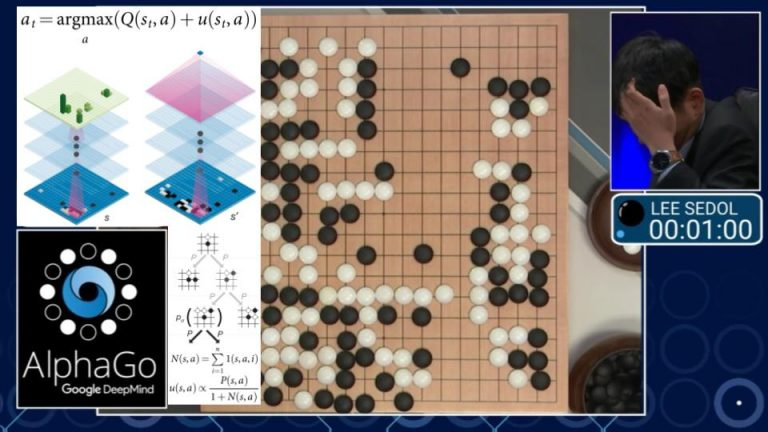
\includegraphics[width=1.8in]{graphics/go-game.jpeg}
%{graphics/adversarial_img_1.png}
\end{minipage}
\begin{minipage}{2.0in}
\centering
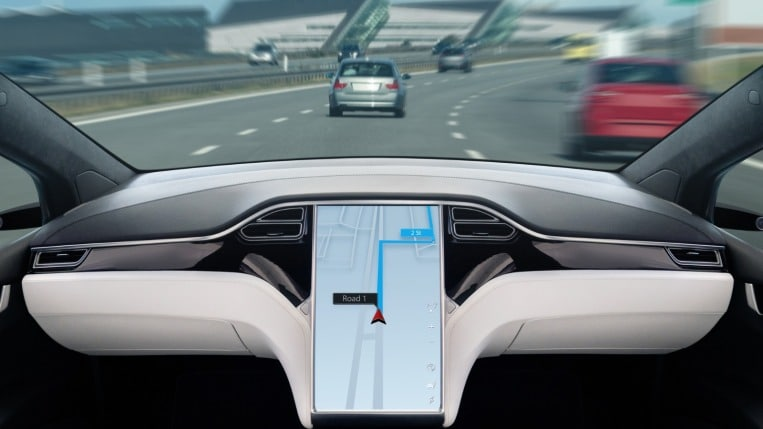
\includegraphics[width=1.5in]{graphics/autonomous-car.jpg}
\end{minipage}
\vfill
\alert{\LARGE\bfseries DNN EVERYWHERE}
\vfill
\begin{minipage}{2.0in}
\centering

\includegraphics[width=1.5in]{graphics/fake-news.jpg}
\end{minipage}
\begin{minipage}{2.0in}
\centering

\includegraphics[width=1.5in]{graphics/covid.jpg}
\end{minipage}
\end{figure}
\end{frame}


\subsection{DNN Problems}
  % but DNNs also have all sorts of problems


\begin{frame}{DNN Problems}
\centering
\includegraphics[width=4in]{graphics/politican-criminals}
\end{frame}

% \begin{frame}
% \centering
% \includegraphics[width=4in]{graphics/obama}
% \end{frame}


\begin{frame}
  \begin{figure}
  \begin{minipage}{2.5in}  
  \centering
  
\includegraphics[width=2.5in]{graphics/bias-gun1}
\end{minipage}
\begin{minipage}{2in}
\centering
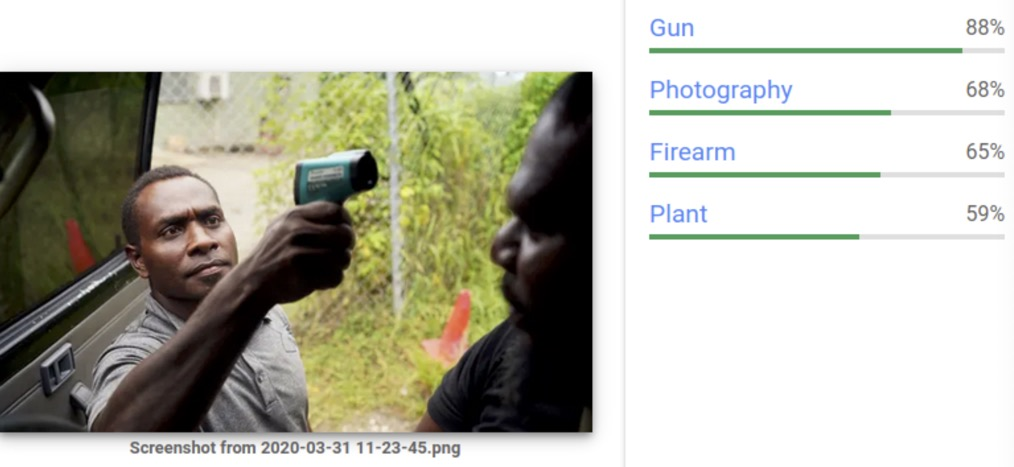
\includegraphics[width=2in]{graphics/bias-gun2}
\end{minipage}
\begin{minipage}{2in}
\centering
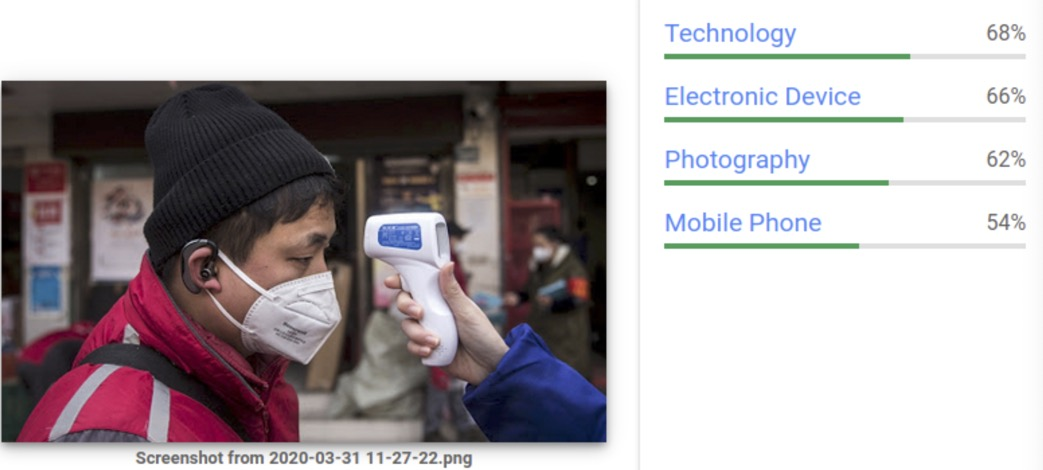
\includegraphics[width=2in]{graphics/bias-gun3}
\end{minipage}
\end{figure}
\end{frame}

\begin{frame}
\centering
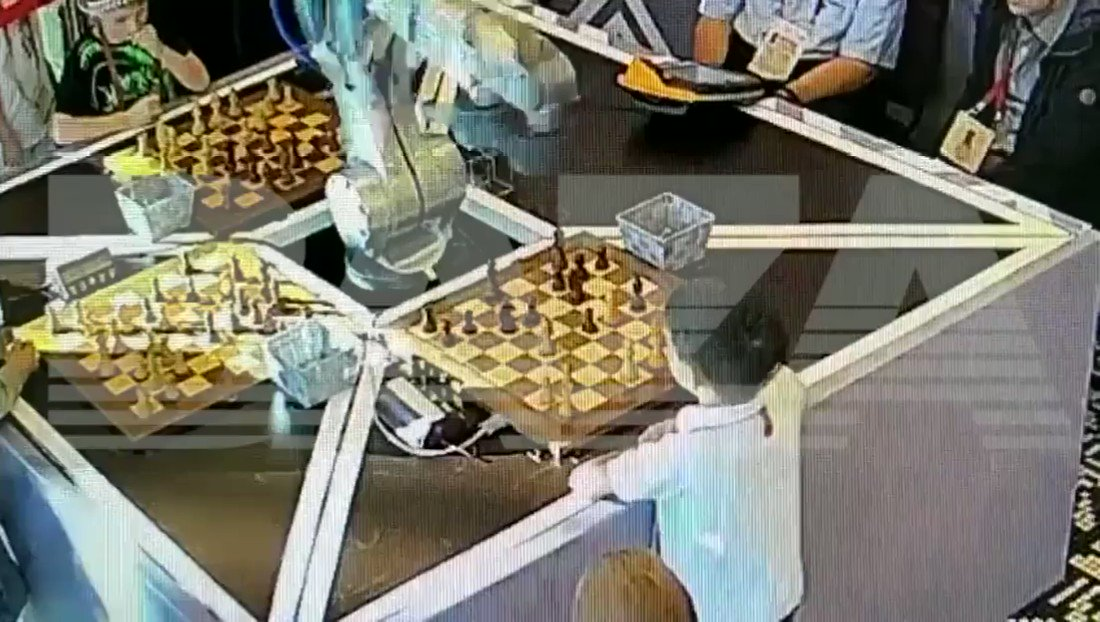
\includegraphics[width=4in]{graphics/break-finger}
\end{frame}

\begin{frame}
\centering
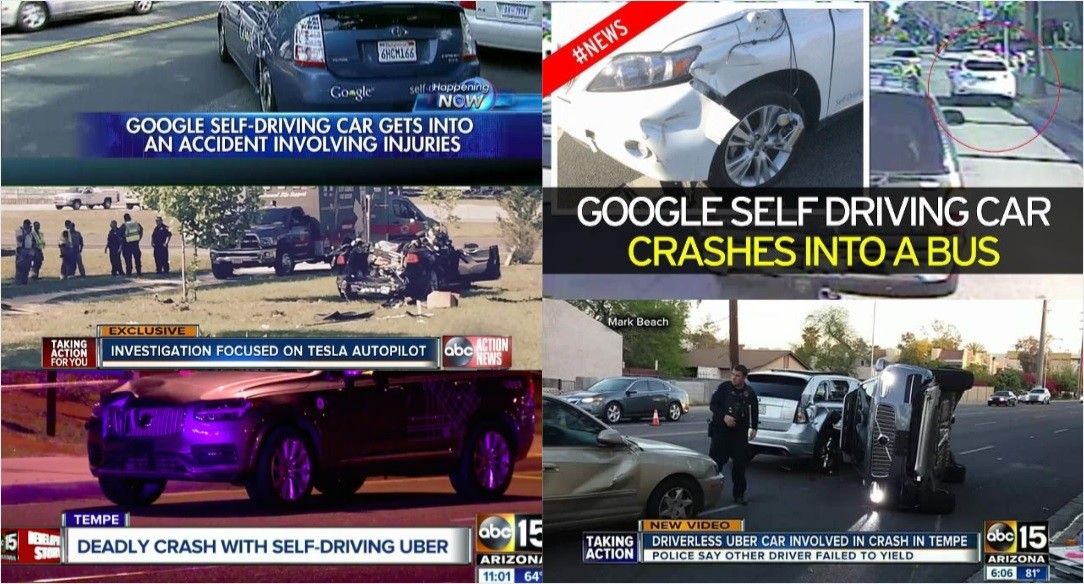
\includegraphics[width=4in]{graphics/car-crashes.jpeg}
\end{frame}

\subsection{Violations}
  % Many possible reasons for these problems,
  % but the most common one is that
  % they violate certain expected properties (robustness and safety)


\begin{frame}{Robustness Properties}
\centering
\includegraphics[width=4.5in]{graphics/adversarial-stoplight.pdf}
\vfill
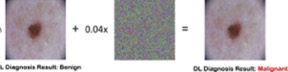
\includegraphics[width=4.5in]{graphics/adversarial-cancer.pdf}
\end{frame}


% \begin{frame}{DNN Problems}
% \centering
% \includegraphics[width=4.5in]{graphics/adversarial-mispell.pdf}
% \end{frame}



% \begin{frame}
% \begin{figure}
% \begin{minipage}{2.0in}
% \centering
% \includegraphics[width=1.7in,height=1.0in]{graphics/adversarial_img_1.png}
% \\{\footnotesize Adversarial Attacks\\~}
% \end{minipage}
% \begin{minipage}{2.0in}
% \centering
% 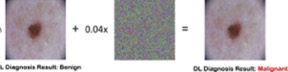
\includegraphics[width=1.5in,height=1.2in]{graphics/adversarial-cancer.jpg}
% \end{minipage}
% \vfill
% \pause
% \alert{\LARGE\bfseries DNN PROBLEMS}
% \vfill
% \begin{minipage}{2.0in}
%   \centering
%   \includegraphics[width=1.5in,height=1.5in]{graphics/adversarial-mispell.jpg}
% \\{\footnotesize First death by AV\\~}  
% \end{minipage}
% \begin{minipage}{2.0in}
% \centering
% \includegraphics[width=1.5in,height=1.0in]{graphics/deadly-crash-self-driving-uber.jpeg}
% \\{\footnotesize First death by AV\\~}
% \end{minipage}
% \end{figure}
% \end{frame}



% \begin{frame}
% \begin{figure}  
% \begin{minipage}{1.0in}
% \centering
% \includegraphics[width=0.85in,height=0.9in]{graphics/bug_wow.jpg}%game
% \\{\footnotesize World of \\Warcraft bug\\~}
% \end{minipage}
% \begin{minipage}{1.0in}
% \centering
% \includegraphics[width=0.85in,height=0.9in]{graphics/bug_therapy.jpg}%airplane
% \\{\footnotesize Therac-25 machines\\X-rays overdose}
% \end{minipage}
% \begin{minipage}{1.0in}
% \centering
% \includegraphics[width=0.90in,height=0.6in]{graphics/deadly-crash-self-driving-uber.jpeg}
% \\{\footnotesize First death by AV\\~}
% \end{minipage}
% \begin{minipage}{1.0in}
% \centering
% \includegraphics[width=0.85in,height=0.9in]{graphics/bug_blackout2.jpeg}%electronic
% \\{\footnotesize North America blackout\\~}
% \end{minipage}
% \end{figure}
%\end{frame}
% \note{
% The world we are living in is increasingly dependent on software.
% We use software for almost everything, playing games, medical treatment, traveling, etc.
% Yet these software that we depend on could be unrealiable.

% Software bugs range from annoying misbehavors causing virtual deaths in computer games to real threats to human lives and other disasterous consequences that affect millions of people
% }


\begin{frame}{Safety Properties}
  \centering
  \includegraphics[width=4.5in]{graphics/deadly-crash-self-driving-uber}
%\emph{Safety requirement}: if the intruder is distant and significantly slower than us, then we stay below a certain threshold (ACAS XU)
\end{frame}

\subsection*{Verification Problem}
\begin{frame}
  \begin{mredblock_nsd}{DNN Verification}
    \textbf{Question}: Given a network $N$ and a property $p$, does $N$ have $p$?
    \begin{itemize}
    \item $p$ often has the form $\greenalert{P} \Rightarrow \alert{Q}$ (precondition $\greenalert{P}$, postcondition $\alert{Q}$)
    \end{itemize}
    
    % \end{itemize}
    \textbf{Answer}: Yes / No
    \vfill
    \pause
    \begin{mgreenblock_nsd}{Simple DNN with ReLU}
    \centering
    \includegraphics[width=2.2in]{graphics/dnn.pdf}
    
      \begin{itemize}
      \item E.g., $x_3 = \max(-1x_1 + -0.5x_2, 0)$
        \pause
      \item Valid: $\greenalert{x_1 \in [-1,1] \land x_2\in[-2,2]} \Rightarrow \alert{x_5 \le 0}$
      \item Invalid: $\greenalert{x_1 \in [-1,1] \land x_2\in[-2,2]} \Rightarrow \alert{x_5 > 0}$
      \end{itemize}
    \end{mgreenblock_nsd}
    
    %\begin{itemize}
    % \item Encoded as a SAT problem: UNSAT (Yes), SAT (No, counterexample)
    %     \end{itemize}
    %     % \begin{itemize}
    %     % \item Networks: Feed-forward, Recurrent, Residiual, Convolution, etc
    %     % \item Properties: various types of properties
    %     %   \begin{itemize}
    %     %   \item \alert{Safety} specifications to avoid collision in unmanned aircraft 
    %     %   \item Adversarial \alert{robustness}: a small input perturbation does not cause major spikes in the DNN's 
    %     %   \end{itemize}
    %     % \end{itemize}
      \end{mredblock_nsd}
\end{frame}



%% \begin{frame}{Example}
  
%% \end{frame
%}



% \begin{frame}{Encoding Properties}
  
%   % \begin{mredblock}{}
%     \begin{center}
%       \includegraphics[width=3.2in]{graphics/dnn.pdf}
%     \end{center}
    

    % output $x_5 \le 0$ for any inputs $x_1 \in [-1,1], x_2\in[-2,2]$
  %\end{mredblock}
  
    % \begin{itemize}
    %     \item \alert{valid} property:
    %     % \begin{itemize}
    %     %     \item  \emph{local robustness}:  the output remains within some bound when individual inputs are close within certain regions
    %     % \end{itemize}
    %     \item \alert{invalid} property:  $x_5 > 0$ for similar inputs
    %     % \begin{itemize}
    %     %     \item cex: $\{x_1=0.0, x_2=-2.0\}$: network evaluates to $x_5=-1.0$
    %     % \end{itemize}
    %     \end{itemize}
%\end{frame}

% \begin{frame}

%     % \begin{mgreenblock}{Sound and Complete}
%     %   \begin{itemize}
%     %     \item \emph{Sound:} if the verifier proves $N$ has $p$, then $p$ is a property of $N$
%     %     \item \emph{Complete:} if $p$ is a property of $N$, then the verifier proves that
%     % \end{itemize}
%     % \end{mgreenblock}    
% \end{frame}



%% \section{Existing Verification Work}
%% \begin{frame}{Abstraction}
  
%%   \begin{itemize}
%%         \item Overapproximate computation (e.g., ReLU) using abstract domains
%%           \begin{itemize}
%%           \item interval, zonotopes, polytopes
%%           \end{itemize}
%% \includegraphics[width=4in]{graphics/abs1.pdf}          
%% \pause
%%         \item Scale well, but \emph{loose precision} (producing spurious cex's)
%%             \begin{itemize}
%%             \item Newer work: iterative refine abstraction to filter spurious cex's
%%             \end{itemize}
%%   \end{itemize}  
%% \end{frame}


%% \begin{frame}{Constraint Solving}
%%   \centering
%%   \includegraphics[width=2.5in]{graphics/verifying-arch.pdf}
%%   \vfill
%%   \pause
  
%%   \begin{itemize}
%%   \item Transform DNN verification into a constraint (satisfiability) problem
%%     \begin{itemize}
%%     \item To prove $N \Rightarrow p$ (where $p$ is $P \Rightarrow Q$) 
%%       \begin{itemize}
%%       \item check if $\neg{(N \Rightarrow (P \Rightarrow Q))}$, i.e., $N \land P \land \neg{Q}$ is satisfiable
%%       \item \alert{UNSAT}: $p$ is a property of $N$
%%       \item \alert{SAT}:  $p$ is not a property of $N$ (also give counterexample inputs satisfiying $P$ but not $Q$)
%%       \end{itemize}
%%     \end{itemize}
%%     \pause
%%   \item Solve the constraint
%%     \begin{itemize}
%%     \item SMT solvers or customized simplex
%%     \item MILP-based solvers
%%     \end{itemize}
%%   \item \alert{Scalability} is a {\large Huge} problem
%%   \end{itemize}  
%% \end{frame}
      


\section{\tool{}}

\begin{frame}
  \begin{mredblock_nsd}{Complexity}
    \begin{itemize}
    \item DNN Verification (with ReLU activation) is \alert{NP-Complete}
    \item \textbf{Scalability} is the main problem
    \item State-of-the-art verification tools: networks with \emph{138M} of parameters, 160K inputs
    \item Real-world networks: \emph{3.5B} parameters, 1.2M of inputs
    \end{itemize}
  \end{mredblock_nsd}
  \pause
  \begin{mblockvu}{}
    \centering
    \alert{SCALABILITY is CRUCIAL}!
  \end{mblockvu}
\end{frame}


\begin{frame}
  \begin{mredblock_nsd}{SAT Solving}
    Many applications: scheduling, hardware model, checking, program analysis, software testing, verification, synthesis
    \pause
  \begin{columns}[c]
    \begin{column}{0.20\linewidth}
      \centering
      \includegraphics[width=1.2in]{graphics/wantedpnp.jpeg}
    \end{column}
    \hfill
    \begin{column}{0.70\linewidth}
      \begin{itemize}
      \item '61: DPLL algorithm (by Davis, Putnam, Logemann, Loveland)
      \item '71: 1st NP-Complete problem (S. Cook)
      \item '92-'93: local/random search
      \item '96-: conflict-driven clause learning (CDCL)
        \begin{itemize}
        \item major \alert{breakthrough} in late 90s - early 200
        \item millions of constraints
        \end{itemize}
      \item '02: DPLL(T):  SMT solving
      \item '06: Yices , '08: Z3, ..
      \item '17: DNN verification is NP-Complete, Reluplex/Marabou (DPLL/simplex-based verifier)
      \end{itemize}
  \end{column}
  \end{columns}      
    \end{mredblock_nsd}

\end{frame}

%% \begin{frame}{\tool{}: Our Current Work}
%%   %split into 2 columns, left is the NeralSAt arc and DNN example
%%   \begin{columns}[c]
%%     \begin{column}{0.4\linewidth}
%%       \centering
%%       \includegraphics[width=2in]{graphics/dpll.pdf}
%%     \end{column}
%%     \hfill
%%     %\pause
%%     \begin{column}{0.5\linewidth}
%%       \begin{itemize}
%%       \item Works as a constraint solver
%%       \end{itemize}
%%     \end{column}
%%   \end{columns}
%% \end{frame}




% \begin{frame}{\tool{}: Our DNN Constraint Solver}
%   %split into 2 columns, left is the NeralSAt arc and DNN example
%   \begin{columns}[c]
%     \begin{column}{0.27\linewidth}
%       \centering
%       \includegraphics[width=1.7in]{graphics/dpll.pdf}
%     \end{column}
%     \hfill
%     %\pause
%     \begin{column}{0.57\linewidth}
%       % \begin{mredblock}{\tool{}: take as input $\alpha$}
%       %   \begin{itemize}
%       %   \item Return \alert{UNSAT} if $\alpha$ is unsatisfiable
%       %   \item Otherwise return \alert{SAT} and a satisfying assignment
%       %   \end{itemize}
%       % \end{mredblock}
%       \begin{mredblock_nsd}{Use \tool{} to prove $N\Rightarrow (P \Rightarrow Q)$}
%         \begin{itemize}
%         \item Call \tool{}($N \land P \land \neg{Q}$)
%         \item Return \alert{UNSAT} or \alert{SAT} (and counterexample)
%         \end{itemize}
%       \end{mredblock_nsd}
%     \end{column}
%   \end{columns}

%       \begin{mblockvu}{}
%         \textbf{Insight:} combines \alert{conflict clause learning} in SAT solving and \alert{abstraction} for scalability
%       \end{mblockvu}  
% \end{frame}

\begin{frame}{Example: Simple FNN with ReLU activation}
  \begin{center}
    \includegraphics[width=3in]{graphics/dnn.pdf}
  \end{center}

  To prove $f: x_1 \in [-1,1] \land x_2\in[-2,2] \Rightarrow \alert{x_5 \le 0}$:
  \begin{itemize}
  \item Use \tool{} to check if $\neg{f}$ is satisfiable
  \item $\tool(N \land x_1 \in [-1,1] \land x_2\in[-2,2] \land \alert{x_5 > 0})$
  \item \tool{} returns \alert{UNSAT}, indicating $f$ is valid
  \end{itemize}
\end{frame}


% % \begin{frame}{GenTree: Dynamic Interaction Discovery \mypub{FSE'16, ICSE'21}}
% %   \begin{columns}[b]
% %     \begin{column}{0.52\linewidth}
% %       \begin{itemize}
% %         \item Use \alert{decision trees} to represent interactions\\  
% %           \begin{center}
% %             \includegraphics[width=1\linewidth]{graphics/ct1}\\
% %           \end{center}
% %         \item \pause \alert{C5$_i$}:  new classification algorithm
% %         \end{itemize}
% %     \end{column}
% %     \hfill
% %     \pause
% %     \begin{column}{0.48\linewidth}
% %       Iterative approach\\
% %       \begin{center}
% %         \includegraphics[width=0.8\linewidth]{graphics/igen2}  
% %       \end{center}
% %     \end{column}
    
% %   \end{columns}
% % \end{frame}

%% \begin{frame}
%%   %split into 2 columns, left is the NeralSAt arc and DNN example
%%   \begin{columns}[c]
%%     \begin{column}{0.42\linewidth}
%%       \centering
%%       \includegraphics[width=1.7in]{graphics/dpll.pdf}
%%       \begin{mblock}{}
%%       \includegraphics[width=1.7in]{graphics/dnn.pdf}
%%       {\footnotesize $x_1  \in [-1,1], x_2 \in [-2, 2], \alert{x_5 > 0}$}
%%       \end{mblock}
%%     \end{column}
%%     \hfill 
%%     %\pause
%%     \begin{column}{0.6\linewidth}
%%       \begin{mredblock_nsd}{Boolean Abstraction}
%%       \begin{itemize}
%%       \item Create 2 \alert{boolean} variables $v_3$ and $v_4$ to represent \emph{activation status} of $x_3, x_4$
%%         \begin{itemize}
%%           \item $v_3=T$ means $x_3$ is active, $-x_1-0.5x_2-1>0$
%%           \end{itemize}
%%           \pause
%%       \item Form two \alert{clauses} $\{v_3 \lor \overline{v_3} \;;\; v_4 \lor \overline{v_4}\}$
%%       \item \alert{Find boolean values for $v_3,v_4$} that satifies the clauses and their implications
%%       \end{itemize}
%%     \end{mredblock_nsd}
%%     \end{column}
%%   \end{columns}
%% \end{frame}

%% \begin{frame}
%%   \begin{columns}[c]
%%     \begin{column}{0.42\linewidth}
%%       \centering
%%       \includegraphics[width=1.7in]{graphics/dpll.pdf}
%%       \begin{mblock}{}
%%       \includegraphics[width=1.7in]{graphics/dnn.pdf}
%%       {\footnotesize $x_1  \in [-1,1], x_2 \in [-2, 2], \alert{x_5 > 0}$}
%%       \end{mblock}
%%     \end{column}
%%     \hfill 
%%     %\pause
%%     \begin{column}{0.6\linewidth}
%%       \begin{mredblock_nsd}{Iteration 1}
%%       \begin{itemize}
%%       \item Use \textbf{abstraction} to approximate upperbound $x_5 \le 0.55$ (from $x_1 \in [-1, 1], x_2 \in [-2,2]$)
%%         \pause
%%       \item \textbf{Deduce} $x_5 > 0$ \emph{might be} feasible
%%         \pause
%%       \item \textbf{Decide} \alert{$v_3=F$} (randomly)
%%         \begin{itemize}
%%           \item new constraint $-x_1-0.5x_2-1 < 0$
%%         \end{itemize}
%%       \end{itemize}
%%     \end{mredblock_nsd}
%%     \end{column}
%%   \end{columns}
%% \end{frame}


%% \begin{frame}
%%   \begin{columns}[c]
%%     \begin{column}{0.42\linewidth}
%%       \centering
%%       \includegraphics[width=1.7in]{graphics/dpll.pdf}
%%       \begin{mblock}{}
%%       \includegraphics[width=1.7in]{graphics/dnn.pdf}
%%       {\footnotesize $x_1  \in [-1,1], x_2 \in [-2, 2], \alert{x_5 > 0}$}
%%       \end{mblock}
%%     \end{column}
%%     \hfill 
%%     %\pause
%%     \begin{column}{0.6\linewidth}
%%       \begin{mredblock_nsd}{Iteration 2}
%%       \begin{itemize}
%%       \item \textbf{Approximate} upperbound $x_5 \le 0$ (due to additional constraint from $v_3=F$)
%%       \item \textbf{Deduce} $x_5 >0$ infeasible: \alert{CONFLICT}
%%         \pause
%%       \item \textbf{Analyze} conflict, \textbf{backtrack} and erase prev. decision $v_3=F$
%%       \item \textbf{Learn} new clause \alert{$v_3$}
%%         \begin{itemize}
%%           \item $v_3$ will have to be $T$ in next iteration
%%         \end{itemize}
%%       \end{itemize}
%%     \end{mredblock_nsd}
%%     \end{column}
%%   \end{columns}
%% \end{frame}

%% \begin{frame}
%%   \begin{columns}[c]
%%     \begin{column}{0.42\linewidth}
%%       \centering
%%       \includegraphics[width=1.7in]{graphics/dpll.pdf}
%%       \begin{mblock}{}
%%       \includegraphics[width=1.7in]{graphics/dnn.pdf}
%%       {\footnotesize $x_1  \in [-1,1], x_2 \in [-2, 2], \alert{x_5 > 0}$}
%%       \end{mblock}
%%     \end{column}
%%     \hfill 
%%     %\pause
%%     \begin{column}{0.6\linewidth}
%%       \begin{mredblock_nsd}{Iteration 3}
%%       \begin{itemize}
%%       \item \textbf{Decide} \alert{$v_3=T$} (\textbf{BCP}, due to learned clause $v_3$)
%%         \begin{itemize}
%%           \item new constraint $-x_1-0.5x_2-1 > 0$
%%         \end{itemize}
%%         \pause 
%%       \item \textbf{Approximate} new upperbound for $x_5$ (using additional constraint from $v_3=T$)
%%       \item \textbf{Deduce} $x_5 > 0$ might be feasible
%%       \item \textbf{Decide} \alert{$v_4=T$} (randomly)
%%       \item $\vdots$
%%       \end{itemize}
%%     \end{mredblock_nsd}
%%     \end{column}
%%   \end{columns}
%% \end{frame}


%% \begin{frame}
%%   \begin{columns}[c]
%%     \begin{column}{0.42\linewidth}
%%       \centering
%%       \includegraphics[width=1.7in]{graphics/dpll.pdf}
%%       \begin{mblock}{}
%%       \includegraphics[width=1.7in]{graphics/dnn.pdf}
%%       {\footnotesize $x_1  \in [-1,1], x_2 \in [-2, 2], \alert{x_5 > 0}$}
%%       \end{mblock}
%%     \end{column}
%%     \hfill 
%%     %\pause
%%     \begin{column}{0.6\linewidth}
%%       \begin{mredblock_nsd}{After several iterations}
%%       \begin{itemize}
%%       \item \textbf{Learn} clauses $\{v_3, \overline{v_3}\lor v_4, \overline{v_3} \lor \overline{v_4}\}$
%%       \item \textbf{Deduce} not possible to satisfy the clauses
%%         \pause
%%       \item \textbf{Return} \alert{UNSAT}
%%         \begin{itemize}
%%         \item Cannot find inputs satisfying $x_1  \in [-1,1], x_2 \in [-2, 2]$ that cause $N$ to return $x_5>0$
%%         \item Hence, $x_5 \le 0$ holds (i.e., the original property is valid)
%%         \end{itemize}
%%       \end{itemize}
%%     \end{mredblock_nsd}
%%     \end{column}
%%   \end{columns}
%% \end{frame}

% \begin{frame}{Example}
%     % We demonstrate how \tool{} proves that the DNN in Fig.~\ref{fig:dnn} has the safety/robustness property mentioned in \S\ref{sec:background}: for all inputs $x_1 \in [-1, 1], x_2 \in [-2,2]$, the DNN produces the output $x_5 \le 0$.
%     % Thus, we want to show that \emph{no} value assignments to $x_1,x_2$ satisfying the input properties that would result in $x_5 > 0$, the negation of the output property.
    
%     \begin{itemize}
%         \item Boolean abstraction
%         \begin{itemize}
%             \item Create 2 variables $v_3$ and $v_4$ to represent activation status
%             \item Form two clauses $\{v_3 \lor \overline{v_3} \;;\; v_4 \lor \overline{v_4}\}$ 
%         \end{itemize}
%         \item Finding truth assignment for $v_3, v_4$
%         \begin{itemize}
%             \item  Iter. 1, from the input $x_1 \in [-1, 1], x_2 \in [-2,2]$, approximates the upper bound $x_5 \le 0.55$ and deduces output $x_5 > 0$ \emph{might be} feasible, and then continues with a (random) decision $v_3=F$. 
%             \item Iter. 2, determines that, with the new constraint imposed by $v_3=F$, the upper bound is $x_5\le 0$ and thus cannot satisfy $x_5 > 0$. It then analyzes the infeasibility to learn the clause $v_3$ (i.e., $v_3$ must be $T$) and backtracks to the previous decision $v_3=F$ to erase it. 
%             \item Iter. 3, infers $v_3=T$ because of the recently learned clause $v_3$, determines that this assignment is feasible, and continues with a (random) decision $v_4=T$.
%             \item $\dots$
%             \item After 5 iters, learns clauses $\{v_3, \overline{v_3}\lor v_4, \overline{v_3} \lor \overline{v_4}\}$, realizes unsatisfiability, and returns unsat (i.e., the property is valid)
%         \end{itemize}
%     \end{itemize}

%     % First, \tool{} creates two variables $v_3$ and $v_4$ to represent the (pre-ReLU) activation status of the hidden neurons $x_3$ and $x_4$. For example, $v_3=T$ means $x_3$ is \texttt{active}, i.e., $-x_1-0.5x_2-1>0$, and $v_3=F$ means $x_4$ is \texttt{inactive}, i.e.,  $-x_1-0.5x_2-1\le 0$. Next, \tool{} forms two clauses  $\{v_3 \lor \overline{v_3} \;;\; v_4 \lor \overline{v_4}\}$ indicating these variables are either \texttt{active} or \texttt{inactive}.
    
%     % Now, \tool{} searches for truth assignments for activation variables to satisfy the clauses. %(and later check that they also satisfy the constraints of DNN implied by these variables and the properties to be proved).
%     % %We summarize the five iterations \tool{} uses to determine that no such assignment exists (i.e., \texttt{unsat}).


% \end{frame}
\section{Results}
\begin{frame}{\tool{}'s Prototype and Preliminary Results}

    \begin{itemize}
        \item Written in Python (not yet optimized, still under heavy development)
        \item Accept standard DNN formats and specs (e.g., ONNX)
        \item Use \alert{DPLL} + conflict clause learning (\alert{CDCL}) in SAT/SMT solving for clause learning, conflict analysis, non-chronological backtracking
        \item Use the \alert{polytope} abstraction (can be replaced with any other abstractions)
    \end{itemize}
\end{frame}

\begin{frame}{ACAS XU Results (results in seconds)}
  \begin{center}
  \begin{tabular}{crr}
    \footnotesize
    \textbf{Property} & \textbf{\tool{}} & \textbf{Marabou}\\
    \toprule
    $\phi_1$   & 1025.36        & TO (3 hrs)   \\
    $\phi_2^*$ & \textbf{22.84} & 821.41\\
    $\phi_3$ & \textbf{526.77} & 8309.09 \\
    $\phi_4$ & 330.83 & \textbf{133.97} \\
    $\phi_5$ & \textbf{83.51} & 1259.74 \\
    $\phi_6$ & \textbf{127.35} & 250.41\\
    $\phi_7^*$ & \textbf{262.01} &  TO \\
    $\phi_8^*$ & \textbf{0.15} &TO \\
    $\phi_9$ & \textbf{142.00} & TO \\
    $\phi_{10}$ & \textbf{191.99} & 3134.35\\
  \end{tabular}
    \end{center}  

  \pause  
  Much faster than the constraint solver \textbf{Marabou}  
  \begin{itemize}
  \item Promising because \tool{} prototype has \emph{no} optimizations
  \end{itemize}
  \pause
  Slower than \textbf{nnenum} (abstraction-based, VNN-COMP'21 winner)
  \begin{itemize}
  \item \textbf{nnenum} applies a series of \emph{seven} optimizations
  \item comparable if \textbf{nnenum} uses single thread
  \end{itemize}
\end{frame}

%% \section{GNN}
%% \begin{frame}{Analyzing Graph Neural Networks}
%%   \begin{itemize}
%%   \item \tool{} focuses on Feed-forward models
%%     \begin{itemize}
%%     \item Feedfoward, Residual, Recurrent, and Covolutional Networks
%%     \end{itemize}
%%     \pause
%%   \item GNNs are very different
%%   \begin{columns}[c]
%%     \begin{column}{0.35\linewidth}
%%       \centering
%%       \includegraphics[width=2in]{graphics/gnn.png}
%%     \end{column}
%%     \hfill
%%     %\pause
%%     \begin{column}{0.55\linewidth}
%%     \begin{itemize}
%%     \item inputs are \alert{graphs}
%%     \item \alert{dynamic computation} based on input structures
%%     \end{itemize}
  
%%     \end{column}
%%   \end{columns}
%% \item But are very powerful and have many applications
%%   \begin{itemize}
%%   \item COVID-19 detection and vaccine development
%%   \item heuristics for NP-Complete problems
%%   \item Text/Image Classification
%%   \item Recommender systems
%%   \end{itemize}
%%   \end{itemize}
%% \end{frame}

%% \begin{frame}{Transforming GNNs into FNNs}
%%   \begin{itemize}
%%     \item \textbf{Idea}: transform GNNs to FNNs to reuse knowledge and tools
%%     \item \textbf{Challenges}
%%     \begin{itemize}
%%       \item cannot create a single FNN accepting all possible graph inputs
%%       \item cannot create a single FNN for each graph of inputs
%%     \end{itemize}
%%     \pause
%%   \item \textbf{Insight}: extract \alert{influential substructures} for GNN prediction
    
%%     \pause
%%     \centering
%%     \includegraphics[width=3in]{graphics/gnnexplainer.png}  
    
%%   \end{itemize}
%% \end{frame}


%% \begin{frame}{GNN-Infer}
%%   \centering
%%   \includegraphics[width=1.7in]{graphics/substructure-miner.pdf}
%%   \begin{enumerate}
%%   \item \textbf{Obtain} influential substructures from sample graphs using existing tools (e.g., GNNExplainer)
%%     \begin{itemize}
%%     \item Use \alert{graph isomorphism} to check if substructures cover input graphs
%%     \end{itemize}
%%   \item \textbf{Create} an FNN by \alert{unrolling} message passing of the GNN over structuctures
%%     \begin{itemize}
%%       \item Neurons and connections representing computation of message update operation of GNN
%%     \end{itemize}
%%   \item \textbf{Combine} FNNs to represent GNN
%%     \pause
%%   \item \textbf{Applications}
%%     \begin{itemize}
%%     \item Use Prophecy to \alert{infer specifications} of FNN to explain original GNN
%%     \item Use Marabou/nnenum/\tool{} to \alert{verify properties} of GNN
%%     \end{itemize}
%%   \end{enumerate}    
%% \end{frame}


\begin{frame}{Current Work / Future Directions}
  \begin{mredblock_nsd}{Continue development on \tool{} and GNN-Infer}
  \begin{itemize}
  \item Parallize algorithms (e.g., Branch and Bound)
  \item Develop more precise (but still fast) abstraction
  \item Different search heuristics for boolean decisions
  \item Extending existing FNN spec. inference tools for GNN-Infer
  \end{itemize}
  \end{mredblock_nsd}
  \pause
  \begin{mgreenblock_nsd}{Future Directions}
  \begin{itemize}
  \item Support richer specifications    
  \item Mining specifications
  \item Apply formal reasoning (verification, specs. mining) to GNNs
  \item Theory/Foundation, e.g., subsets of DNN verification probs have poly. time alg?
  \end{itemize}
  \end{mgreenblock_nsd}
\end{frame}

\begin{frame}{Impacts}
  \begin{itemize}
  \item NSF CAREER (2023–2028)
  \item Amazon Research Award
  \item ranked 4th in VNN-COMP’23 (the annual neural network verification competition)
  \item featured in SIGBED (Special Interest Group from Embedded Systems)
  \end{itemize}
\end{frame}



\subsection{Build Systems (since 2015, during postdoc)}

\begin{frame}{Impacts}
  \begin{itemize}
  \item Pubs
  \item Funding
    \begin{itemize}
  \item NSF CRII award '20
  \item a UNL Seed award '21;
  \item Facebook unrestricted gift
  \item NSF Formal Methods in the Field (FMiT) '23
    \end{itemize}
  \item Industry adoption: Cybolic used internally at Meta Whatsapp
  \end{itemize}
\end{frame}


\subsection{Invariant Generation and Program Repair (since 2007, during PhD study)}

\begin{frame}{Impacts}
  \textbf{Funding} NSf Medium grant
  
  \textbf{Invariant Generation: the "bread and butter" of my research}
  \begin{itemize}
    \item 15 pubs
    \item Orig DIG: Distinguish Paper Award at ICSE’12
    \item Industry adoption: GammaTech integrated DIG in their Mnemosyne project
    \item DIG’s nonlinear benchmarks are included in SV-COMP
    \item Funding: NSF Medium grant  (2021–2024)
  \end{itemize}


  \textbf{APR}
  \begin{itemize}
  \item GenProg: multiple paper awards; help create and make the field of APR popular
  \item Most Influential Paper Award (at ICSE '19)
  \item Most Impact Award (at GECCO '19)
  \item 2000+ citations
  \item Industry adoption: Facebook, GammaTech, MIT Lincoln Lab
  \item Funding: Army Research 2018--2021
  \end{itemize}
\end{frame}


%% GenProg has received multiple awards, e.g., best papers at ICSE, GECCO, ICST, and the ACM SIGEVO “Humie” gold medal. In 2019, GenProg was recognized with a 10-year IEEE/ACM Most Influential Paper award at ICSE and a 10-year ACM SIGEVO Most Impact Award at GECCO for showing that real-world programs can be repaired automatically and creating the now widely popular APR subfield in Software Engineering. Our APR work also has been used in the industry, including GammaTech and MIT Lincoln Lab. In particular, Facebook has adopted ideas in GenProg to find locate and repair bugs in their Android and iOS apps.
%% In total, my APR research has been cited more than 2000 times as of June’23. This line of research has been funded by the mentioned NSF Medium award (2021–2024) and an Army Research Office (ARO) grant (2018–2021). More recently, we have also patented our work on domain specific APR and are applying external funding for this line of work.

\section{Ending}

\begin{frame}[plain]%{The Problem}
\begin{figure}
\begin{minipage}{1.5in}
\centering
\includegraphics[width=1.2in]{graphics/dino.jpg}
%{graphics/adversarial_img_1.png}
\end{minipage}
\begin{minipage}{2.5in}
  \centering
\alert{\Large\bfseries DynaROARS @ GMU\\ \bluealert{\href{https://dynaroars.github.io}{dynaroars.github.io}}}
\end{minipage}
\vfill
\begin{minipage}{0.7in}
\centering
\includegraphics[width=0.52in,height=0.7in]{graphics/tvn.png}
\caption*{Vu}
\end{minipage}
\begin{minipage}{0.7in}
\centering
\includegraphics[width=0.55in,height=0.7in]{graphics/didier.pdf}
\caption*{Didier}
\end{minipage}
\begin{minipage}{0.7in}
\centering
\includegraphics[width=0.55in,height=0.7in]{graphics/linhan.pdf}
\caption*{Linhan}
\end{minipage}
\begin{minipage}{0.7in}
\centering
\includegraphics[width=0.50in,height=0.7in]{graphics/haiduong.pdf}
\caption*{Hai}
\end{minipage}
\begin{minipage}{0.7in}
\centering
\includegraphics[width=0.52in,height=0.7in]{graphics/kimhao.pdf}
\caption*{KimHao}
\end{minipage}
\end{figure}
\end{frame}


% \begin{frame}
%   \begin{columns}
%     \begin{column}{0.45\linewidth}
%       \begin{mblock}{\includegraphics[width=0.6cm,height=0.5cm]{graphics/mozilla.png}{\small -- Mozilla Developer}}
%         \centering
%         \emph{``Everyday, almost \alert{300} bugs appear [..] far too many for only the Mozilla programmers to handle.''}
%     \end{mblock}
%     \end{column}

%     \begin{column}{0.42\linewidth}
%       \begin{mblock}{}
%       \centering
%       Software bugs annually cost \alert{0.6\%} of the U.S GDP and \alert{\$312} billion to the global economy
%     \end{mblock}
%     \end{column}
%   \end{columns}
%   \vfill
%   \begin{columns}
%     \begin{column}{0.4\linewidth}
%       \begin{mblock}{}
%       \centering
%       Average time to fix a security-critical error:\\
%       \alert{28 days}
%     \end{mblock}
%     \end{column}

%     \begin{column}{0.45\linewidth}
%       \begin{mblock}{}
%         \includegraphics[width=1.00\linewidth]{graphics/bugbounty.jpg}
%       \end{mblock}
%     \end{column}
%   \end{columns}
% \end{frame}
% \note{
%   So we have too many software bugs,

%   And it takes lots of time and effort to fix bugs, so even important bugs take a long time to be patched. 
%   The cost of program defects is enormous, 0.6\% of the US economy annually and  according to a 2013 university Cambridge study, software defects cost over 312 billon US dollars to global economy
%   And lately, many companies such as Google and Facebook are paying strangers to anlayze their code to find and fix problems
% }

% \begin{frame}

% \begin{mblockvu}{}
% {\small \emph{Automated program analysis techniques and tools} can decrease debugging time
%   by an average of \alert{26\%} and \alert{\$41} billion annually}
  
% \end{mblockvu}

% \vfill
% \begin{columns}[T]
%   \begin{column}{0.46\linewidth}
%     \begin{mgreenblock_nsd}{Program Verification}
%       \hfill
%       \includegraphics[width=1.3cm,height=1.5cm]{graphics/programmer_computer_green.png}
%       \hfill
%       \includegraphics[width=1.3cm,height=1.5cm]{graphics/programmer_computer_green.png}
%       \hfill
%     \end{mgreenblock_nsd}
%     {\footnotesize Check if a program meets a given specification}
%   \end{column}
%   \begin{column}{0.46\linewidth}  
%   \begin{mredblock_nsd}{Program Repair}
%       \hfill
%       \includegraphics[width=1.3cm,height=1.5cm]{graphics/programmer_computer_red.png}
%       \hfill
%       \includegraphics[width=1.3cm,height=1.5cm]{graphics/programmer_computer_red.png}
%       \hfill
%     \end{mredblock_nsd}
%     {\footnotesize Fix a buggy program to satisfy a given specification}
%   \end{column}
% \end{columns}  

% \end{frame}
% \note{
%   A main cause for software errors is because we, e.g., the developers, are human, and thus we make mistake.
%   For example we write some program code and think that it does X, but instead it does Y.  
%   Or we forget to check some special cases. 
  
%   For this reason, many research in program lagguages and software engineering are devoted to synthesize and to verify code:  new programming languages are developed that are easier and safer to use, mathematical modeling of computer programs so that we can verify programs formally, smarter IDE and debugging tools, etc. 
  
%   So program verification and repairs are two important research areas in computer science.
%  }

%  \begin{frame}[fragile]
   
% \begin{columns}[T]
%   \begin{column}{0.46\linewidth}
% \begin{mgreenblock_nsd}{Invariant Generation}
% \begin{lstlisting}[xleftmargin=0.30cm,basicstyle=\ttfamily\scriptsize,language=python]
% def intdiv(x, y):
%   q = 0
%   r = x
%   while r $\ge$ y:
%     a = 1
%     b = y
%     while [$\color{red} ??$] r $\ge$ 2b: 
%       a = 2a
%       b = 2b
%     r = r - b
%     q = q + a
%     [$\color{red} ??$]  
%     return q   
% \end{lstlisting}
% {\footnotesize 
%   \begin{itemize}
%     \item Discover \alert{invariant properties} at certain program locations
%     \item Answer the question \alert{\emph{``what does this program do ?''}}
%     \end{itemize}
%     }
% \end{mgreenblock_nsd}
%   \end{column}

%   \pause
%   \begin{column}{0.46\linewidth}
% \begin{mredblock_nsd}{Automatic Program Repair}
% \begin{lstlisting}[xleftmargin=0.30cm,basicstyle=\ttfamily\scriptsize,language=Python]
% def intdiv(x, y):
%   q = 0
%   r = x
%   while r $\cancelto{\color{red} \ne}{\ge}$ y:
%     a = 1
%     b = $\cancelto{\color{red}3*y}{y}$
%     while r $\ge$ 2b:
%       a = 2a
%       b = 2b
%     r = r - b
%     q = q $\cancelto{\color{red}- 2*a}{+ a}$

%   return q
% \end{lstlisting}
% {\footnotesize 
%   \begin{itemize}
%     \item \alert{Localize} errors and \alert{modify} code to fix bugs
%     \item A form of \emph{program synthesis}
%     \end{itemize}
% }
% \end{mredblock_nsd}
% \end{column}
% \end{columns}  

% \end{frame}

% \note{My research is in the area of program verfication and synthesis.
% More specifically, for verification, I concentrate on developing automatic techniques to discover invariant properties of programs.  
% These properties describe the semantics of the program, answering the question ``what is this program doing?''.
% After obtaining these properties, you can see if they match your expectation or required specifications

% For synthesis, I concentrate on template-based synthesis and apply it to repair programs. 
% Instead of creating programs from scratch, I create code under specific form to complete a program. 
% Template-based synthesis can be used to automatic program repair, that is, synthesize patches for buggy programs.

% }

% % \begin{frame}
% %   \begin{mredblock_nsd}{Core Research Areas}
% %     \begin{figure}
% %       \centering
% %       \begin{minipage}{1.2in}
% %         \centering
% %         \includegraphics[width=2.5cm,height=1.8cm]{graphics/discovery.png}
% %         \caption*{\scriptsize Invariant Discovery}
% %       \end{minipage}
% %       \hfill
% %       \begin{minipage}{1.2in}
% %         \centering
% %         \includegraphics[width=2.2cm,height=1.5cm]{graphics/ga.png}
% %         \caption*{\scriptsize Program Repair}
% %       \end{minipage}
% %       \hfill
% %       \begin{minipage}{1.5in}
% %         \centering
% %         \includegraphics[width=2.4cm,height=2cm]{graphics/config.png}
% %         \caption*{\scriptsize Configurable System}
% %       \end{minipage}
% %     \end{figure}    
% %   \end{mredblock_nsd}
% %   \pause
% %   \begin{mgreenblock_nsd}{New Research Directions}
% %     \begin{columns}
% %       \hfill
% %       \begin{column}{0.33\linewidth}
% %         \centering
% %         \includegraphics[width=3cm,height=2.5cm]{graphics/makefile.png}\\
% %         {\scriptsize Unix Build Systems}
% %       \end{column}
% %       \hfill
% %       \begin{column}{0.33\linewidth}
% %         \centering
% %         \includegraphics[width=2.4cm,height=2.2cm]{graphics/iot0.jpg}\\
% %         {\scriptsize IoT systems}
% %       \end{column}
% %       \hfill      
% %       \begin{column}{0.33\linewidth}
% %         \centering
% %         \includegraphics[width=2.4cm,height=2.2cm]{graphics/dnn0.png}\\
% %         {\scriptsize AI-generated Software}
% %       \end{column}
% %       \hfill
% %     \end{columns}
% %   \end{mgreenblock_nsd}
  
% % \end{frame}


% \section{Research}

% \subsection{Invariant Generation}

% \begin{frame}{Outline}
%   \tableofcontents[currentsection,currentsubsection]
% \end{frame}


% \begin{frame}{How We Analyze Programs}
%   \begin{columns}[c]
%     \begin{column}{0.25\linewidth}
%       \centering
%       \includegraphics[width=1.2in,height=1.4in]{graphics/printf1.png}
%     \end{column}
%     \begin{column}{0.65\linewidth}
%       \centering
%       \includegraphics[width=3in,height=1.6in]{graphics/intdiv_printf.png}
%     \end{column}
%   \end{columns}
%   \pause
%   \vfill
%   \begin{columns}[c]
%     \begin{column}{0.4\linewidth}
%     \includegraphics[width=4cm,height=3.5cm]{graphics/intdiv_assertions.png}
%   \end{column}

%   \begin{column}{0.5\linewidth}
%       \begin{mblock}{\includegraphics[width=0.6in,height=0.4in]{graphics/udacity.png}{\small ~-- Software Testing course}}
%         \centering
%         \emph{\small ``GCC: ~9000 assertions,\\ 
%           LLVM: ~13,000 assertions [..]\\
%           1 assertion per 110 loc''}
%     \end{mblock}
%   \end{column}
%   \end{columns}
% \end{frame}
% \note{
%   Most of us here have some experience in coding. How do we analyze programs ?  how do we figure out a difficult piece of code ?  

%   A popular and straight forward way is simply outputtings values of the variables at various locations in the programs.  And then run the programs on some inputs and analyze those outputs or traces to figure out what the program is doing.

%   Any perhaps many of us put assertions in our code, we believe that at something must be true at those locations.
  
%  The figure on the right, is from a course at Udacity, showing us that assertions are used frequently in real-world, large, and mature software projects such as Gnu Compiler or LLVM.  On average, there's about 1 assertion per 110 line of code, (including empty lines).
% }


% \begin{frame}[fragile]

%   \begin{mblock}{}
%     \centering
%     \emph{``\alert{program invariants} are asserted properties, such as relations among variables, at certain locations in a program''}
%   \end{mblock}
%   \vfill

% \begin{columns}
%   \begin{column}{0.50\linewidth}
%     \includegraphics[width=1.0\linewidth]{graphics/assertion_error.png}
% \end{column}
% \begin{column}{0.45\linewidth}
%   \begin{mredblock}{Uses}
%   \begin{itemize}
%   \item verify programs
%   \item help understand programs
%   \item reveal interesting, unexpected properties
%   \item debug (locate errors) %see the picture
%   \item documentations
%   \item \dots
%   \end{itemize}
%   \end{mredblock}
% \end{column}
% \end{columns}
% \end{frame}

% \note{
% Program invariants essentially describe the behaviors of the programs in a compact and precise ways such as a mathematical formula.  For example, loop invariants capture the computation of the loops.

% Invariants allow us understand programs and verify if programs behave as expected.

% They are mainly designed for automatic and formal program verification.  If you take any programming analysis then you will learn about Floyd-Hoare semantics which allows partial correctness verification of programs using pre and post conditions and loop invariants.

% They also help locate errors, assertions tell us where some properties are violated

% Invariants are also used to provide precise program documentation instead of vague English description.

% Other uses for invariants including compiler optimization, compilers use invariants to figure what the code is doing so that it can optimize that code,  loop inv code motion, constant progations. 
% }

% \begin{frame}[fragile]{Approaches to Finding Invariants}
%   \begin{columns}[T]
%     \begin{column}{0.34\linewidth}
%       \vspace{0.1in}
%       \usebox{\intdivz}
%     \end{column}
%     \begin{column}{0.62\linewidth}
%       \begin{mblueblock_nsd}{Static Analysis}
%         {\small
%           \begin{itemize}
%           \item Analyze source code directly
%           \item Pros: guaranteed results
%           \item Cons: computationally intensive, infer simple invariants
%           \end{itemize}
%         }
%         \end{mblueblock_nsd}
%     \end{column}
%   \end{columns}

%   \pause
%   \begin{columns}
%     \begin{column}{0.34\linewidth}
%       \begin{center}
%         {\scriptsize
%           \begin{tabular}{c  c | c  c }
%             $x$&$y$&$q$&$r$\\
%             \midrule
%             0   &    1 &    0 &  0 \\
%             1   &    1 &    1 &  0 \\
%             3   &    4 &    0 &  3 \\
%             8   &    1 &    8 &  0 \\
%             15  &    5 &    3 &  0 \\
%             20  &    2 &   10 &  0 \\
%             100 &    1 &  100 &  0 \\
%             %100 &   10 &   10 &  0 \\
%             &\vdots&\vdots&
%           \end{tabular}
%         }
%       \end{center}
%     \end{column}
%     \begin{column}{0.62\linewidth}
%       \begin{mgreenblock_nsd}{Dynamic Analysis}
%         {\small
%           \begin{itemize}
%           \item Analyze program traces 
%           \item Pros: fast, source code not required
%           \item Cons: results depend on traces, might not hold for all runs
%           \end{itemize}
%         }
%       \end{mgreenblock_nsd}
%     \end{column}
%   \end{columns}
% \end{frame}

% \note{
% The study of invariants, more specifically, techniques to automatically find program invariants, is a major research area in the fields of program analys and formal methods for over three decades. 

% Invariants can be identified from programs using static analysis.  Static analysis inspects program code directly, it analyzes the effects of all program constructs to considers all possible program paths on all inputs.
% Thus they have the advantage of discovering sound results that are valid for any program run and input. But the requirement for being sound leads to expensive computation, especially when having to analyze large and complex programs.  

% On the other hand, dynamic analysis, as we have seen, using execution traces, does not have soundness guarateed.  The results are only candidate invariants - they are correct with respected to the observed runs and might not hold for all runs on all inputs.  However, the sacrifice of soundness makes dynamic analysis more efficient,  more practical, and scales well to real-world and complex program.
% }




% \newcommand{\intdivtraces}[1]{
%       \begin{column}{#1\linewidth}
%         \footnotesize
%         \centering
%         \begin{tabular}{c  c || c  c  c c}
%           $x$&$y$&$a$&$b$&$q$&$r$\\
%           \midrule
%           \alert{15}& \alert{2}& 1& 2& 0& 15\\
%           \alert{15}& \alert{2}& 2& 4& 0& 15\\
%           \alert{15}& \alert{2}& 1& 2& 4& 7\\
%           \midrule
%           \alert{4}& \alert{1}& 1& 1& 0& 4\\
%           \alert{4}& \alert{1}& 2& 2& 0& 4\\
%         \end{tabular}
%       \end{column}
% }
% \begin{frame}[fragile]{Example}

%   \begin{figure}
%     \begin{columns}[T]
%       \begin{column}{0.4\linewidth}
%         \usebox{\intdivsimple}
%       \end{column}
%       \pause
%       \hspace{0.05in}
%       \intdivtraces{0.50}
%     \end{columns}
%   \end{figure}

%   Invariants at \alert{L}: $b=ya, ~x=qy+r, ~r \geq 2ya$\\

% \end{frame}

% \note{***

% Let's say we want to know the semantics of this integer division algorithm.
% More specifically, we want to know the invariants of the inner loop, that is, relations of the variables in scope at location L, the entrance of the loop.

% So dyn analysis works on program traces, which are captured by running the program against test inputs.
% We run this program on test inputs and capture the traces representing the values of the six variables in scope at L. For example, when running on the input x=15,y=2, we obtain this set traces.  when running on input x=4,y=1, we obtain this set of traces.

% Note that dynamic analysis works directly from traces and doest not require src code (this is just for illustration purpose).

% From these traces, DIG *automatically* generates these relations representing the semantics of the inner loop of this program.
% For example, the invariant in the middle essentially states that this program does integer division (dividen x equals to quotient q times divisor y  + remainder r).
% ** So if you don't know about this program, than these invariants give some clues that it's doing some sort of division.
% ** If you expect that the program is doing division, then seeing these invariants give you more confidence that the program is doing division.
% Note These invariants are nonlinear and cannot be discovered by current dynamic analysis techniques.
% }


% \begin{frame}%{Polynomial Relations}

%   \begin{mblueblock}{DIG discovers polynomial relations of the forms}
%     {\footnotesize
%     \[
%     \begin{array}{rlr}
%       \alert{\text{Equalities}}&c_0 + c_1x_1 + c_2x_n + c_3x_1x_2 + \dots + c_mx_1^{d_1}\dots x_n^{d_n} = 0&\\[.3cm]
%       \alert{\text{Inequalities}}&c_0 + c_1x_1 + c_2x_n + c_3x_1x_2 + \dots + c_mx_1^{d_1}\dots x_n^{d_n} \ge 0,& c_i \in \mathbb{R}
%     \end{array}
%     \]
%   }
%   \end{mblueblock}

%   \vspace{\fill}
%   {\small Examples}
%   {\footnotesize
%     \[
%     \begin{array}{rl}
%       \text{cubic}        & z - 6n = 6,\;  \frac{1}{12}z^2 - y - \frac{1}{2}z = -1\\[.2cm]
%       \text{extended gcd} & \gcd(a,b)= ia+jb\\[.2cm]
%       \text{sqrt}         & x+\varepsilon \ge y^2 \ge x - \varepsilon\\[.2cm]
%     \end{array}
%     \]
%   }

%   \pause
%   \vspace{\fill}
%   \begin{mredblock_nsd}{Method}
%     \begin{itemize}
%     \item \alert{Equalities}: solve equations
%     \item \alert{Inequalities}: construct polyhedra
%     \end{itemize}
%   \end{mredblock_nsd}
% \end{frame}
% \note{
%   For polynomials, DIG supports (potentially nonlinear) equalities as well as inequalities among numerical variables under these forms.
  
% These are some example nonlinear invariants that DIG generates from programs computing cubic, gcd, and sqrt.

% To find equality invariants: DIG essentially generates equations from traces and uses standard equation solvers to solve them.

% For inequalities: we build a polyhedron over trace points and the facets of the polyhedron represent the inequality constraints.
% }



% \begin{frame}[fragile]{Example}

%   \begin{figure}
%     \begin{columns}[T]
%       \begin{column}{0.4\linewidth}
%         \usebox{\intdivsimple}
%       \end{column}
%       \hspace{0.05in}
%       \intdivtraces{0.50}
%     \end{columns}
%   \end{figure}

%   Invariants at \alert{L}: $\alert{b=ya, ~x=qy+r}, ~r \geq 2ya$

% \end{frame}

% \note{Let's see a walk through to generate nonlinear equalities for this program (highlighted in red)}


% \begin{frame}{Finding Nonlinear Equations using Linear Equation Solving}

%   \begin{columns}[T]
%     \hspace*{-1cm}
%     \begin{column}{.70\linewidth}
%       \vspace{-0.2cm}
%       \begin{itemize}
%       \item<2-> Terms and degrees
%         {\footnotesize
%           \begin{eqnarray*}
%             &V = \alert<2>{\{r,y,a\}};~\text{\tt deg} = 2&\\
%             &\downarrow&\\
%             &\alert<4>{T=\{1,r,y,a,ry,ra,ya,r^2,y^2,a^2\}}&\\
%             &\only<3>{T=\{\dotsc,\alert{\log(r)},\alert{a^y},\alert{\sin(y)},\dotsc\}}&
%           \end{eqnarray*}
%         }

%         \vspace{-0.60cm}
%       \item<4-> Nonlinear equation template
%         {\footnotesize
%           \begin{equation*}
%             \qquad\qquad \alert<4>{c_1+c_2r+c_3y+c_4a+c_5ry+c_6ra+c_7ya+c_8r^2+c_9y^2+c_{10}a^2 = 0}
%           \end{equation*}
%         }

%         \vspace{-0.20cm}
%       \item<5-> System of \alert{linear} equations
%         {\footnotesize
%           \begin{eqnarray*}
%             \qquad\text{trace 1}&:& \{r=15,y=2,a=1\}\\
%             \qquad\text{eq 1}&:& c_1 + 15c_2 + 2c_3 + c_4 + 30c_5 + 15c_6 + 2c_7 + 225c_8 + 4c_9 + c_{10} = 0\\
%             \qquad&\vdots&
%           \end{eqnarray*}
%         }

%         \vspace{-0.50cm}
%       \item<6-> Solve for coefficients $\alert{c_i}$
%         {\footnotesize
%           $$
%           V= \alert<6>{\{x,y,a,b,q,r\}};~\text{\tt deg} = 2 \qquad \longrightarrow \qquad \alert{b=ya, x=qy+r}
%           $$
%         }

%       \end{itemize}
%     \end{column}

%     \begin{column}{.20\linewidth}
%         \hspace*{-0.8cm}
%         \vspace*{-0.3cm}
%         \scriptsize
%         \centering
%         \begin{tabular}{c  c || c  c  c c}
%           \textcolor<2-5>{lightgray}{$x$}& \alert<2-5>{$y$}&\alert<2-5>{$a$}&\textcolor<2-5>{lightgray}{$b$}&\textcolor<2-5>{lightgray}{$q$}&\alert<2-5>{$r$}\\
%           \midrule
%           \textcolor<2-5>{lightgray}{15} & \textbf<5>{\alert<5>{2}}& \textbf<5>{\alert<5>{1}}& \textcolor<2-5>{lightgray}{2}& \textcolor<2-5>{lightgray}{0}& \textbf<5>{\alert<5>{15}}\\
%           \textcolor<2-5>{lightgray}{15} & 2& 2& \textcolor<2-5>{lightgray}{4}& \textcolor<2-5>{lightgray}{0}& 15\\
%           \textcolor<2-5>{lightgray}{15} & 2& 1& \textcolor<2-5>{lightgray}{2}& \textcolor<2-5>{lightgray}{4}& 7\\
%           \midrule
%           \textcolor<2-5>{lightgray}{4}  & 1& 1& \textcolor<2-5>{lightgray}{1}& \textcolor<2-5>{lightgray}{0}& 4\\
%           \textcolor<2-5>{lightgray}{4}  & 1& 2& \textcolor<2-5>{lightgray}{2}& \textcolor<2-5>{lightgray}{0}& 4\\
%         \end{tabular}
%     \end{column}


%   \end{columns}
% \end{frame}

% \note{
% First thing we do generate a set of terms to represent polynomials over variables. For example, if the set of variables is {r,y,a} and we are just interested in polynomials of 2nd degree, then we generate this set T of 10 terms.  The second degree used here is just an example,  you can use higher degree 3,4,5 etc.
%   You can also use terms to represent other functions such as log, exponential, sin, cosine, etc. For simplicity, we don't use these functions for our illustrations.

%   Next, we generate an equation template .. by combining the terms with unknown coefficients.

%   This nonlinear equation template is then instantiated over the traces and become a linear equation.  For example, with this trace 1, we obtain this equation 1.

%   Instantiating set of traces will give us a set of linear equations.  From here, we use a standard equation solver to solve for the unknown coefficients.

%   The main idea here is that we reduce the problem of finding nonlinear equations into solving linear equations by instantiating nonlinear polynomial terms with traces.

%   At the end, applying this technique to our running cohen integer division example with six variables and using degree 2, we obtain this set of quadratic relations}

% \begin{frame}{Geometric Invariant Inference}

%   % \begin{itemize}
%   % \item Treat trace values as points in multi-dimensional space

%   % \item Build a \alert{convex hull} (polyhedron) over the points

%   % \item Representation of a polyhedron: a \alert{conjunction} of inequalities

%   % \pause
%     \begin{figure}
%       \hfill
%       \begin{minipage}{0.22\linewidth}
%           \scriptsize
%         \centering
%           \begin{tabular}{rr}
%             $x$&$y$\\
%             \midrule
%             -2 & 1\\
%             -1 &-1\\
%              1 &-3\\
%              2 & 0\\
%              3 &-2\\
%              5 & 2
%            \end{tabular}
%            \\{\scriptsize program traces}
%       \end{minipage}
%       \hfill
%       \geoshapes{}{\scriptsize trace points\\in 2D}{0.25}
%       \hfill
%       \geoshapes{
%         \draw[mgeoshape] (-2,1) -- (5,2) -- (3,-2) -- (1,-3) -- (-1,-1) -- cycle;
%       }{\scriptsize polygon\\$c_1x+c_2y\ge c$}{0.25}
%       \hfill
%     \end{figure}

%     \pause
%   %\item Support simpler shapes (decreasing precision, increasing efficiency)
%     \begin{figure}
%       \hfill
%       \geoshapes{\draw[mgeoshape] (-2,1) -- (-1,2) -- (5,2) -- (5,0) -- (2,-3) -- (1,-3) -- (-2,0) -- cycle;
%       }{\scriptsize octagon\\$\pm x \pm y \ge c$}{0.25}
%       \hfill
%       \geoshapes{\draw[mgeoshape] (-2,1) -- (-1,2) -- (5,2) -- (5,0) -- (2,-3) -- (-2,-3) -- cycle;}
%       {\scriptsize zone\\$x-y\ge c$}{0.25}
%       \hfill
%       \geoshapes{\draw[mgeoshape] (-2,2) -- (5,2) -- (5,-3) -- (-2,-3) -- cycle;}
%       {\scriptsize box\\$\pm x,y\ge c$}{0.25}
%       \hfill
%       \geoshapes{\draw[mgeoshape] (-2,-3) -- (-2,1) -- (0,1) -- (1,2) -- (5,2) -- (3,0) -- (3,-2) -- (2,-3) -- (1,-3) -- cycle;}
%       {\scriptsize weak max-plus (\bluealert{non-convex})}{0.25}
%       \hfill
%     \end{figure}

%   %\end{itemize}
% \end{frame}
% \note{
%     To find inequalities, we use ideas from convex geometry.
%     This method treats terms representing trace values as points in multi-dim space
%     Then builds a polyhedron representing a convex hull enclosing these points.
%     This polyhedron is represented by a set of linear inequalities

%     In this example, we have a set of program traces over 2 integer variables x and y, we represent them as points in 2 dimensional space and build a convex hull, a bounded convex polygon, over them.
%     Just a reminder, a region is convex if lines btw any 2 points in that region are also in the region.
%     We got this polygon with 5 facets and obtain a cojunction of 5 inequalities over 2 variables x and y.
%     This method of building a convex polyhedron produces a set or conjunction of inequality relations over the traces.

% Building polyhedra is expensive, depending on the number of terms and the number of points.

% This leads us to consider simpler convex geometric shapes represeting simpler inequality invariants (increase precision, increase complexity).
% Even though these invariants are more restricted, e.g., only involve 2 variables, they are computed very efficiently and they are useful in detecting bugs in flight control software, performing array bounds and memory leaks checking

% So this technique of building polyhedra gives set, or conjunction, of formulas.  For example, an octagon gives 8 conjuncts representing the eight sides of an octagon.
% }

% \begin{frame}

%   \begin{mblock}{}
%   \alert{Symbolic States}: logical formulae representing program semantics
%     \begin{itemize}
%     \item \textbf{path conditions} and \textbf{mappings} from variables to symbolic values
%     \item obtained using a symbolic execution tool
%     \end{itemize}
%   \end{mblock}
%   \vfill
%   \centering
%   \includegraphics[width=0.80\linewidth,height=5cm]{graphics/ssft2021_arch.pdf}
%   \vfill
%   \pause
%   \begin{itemize}
%   \item \greenalert{Dynamic Inference}: learn \emph{candidate} invariants under different templates from concrete states (execution traces)
%   \item \alert{Symbolic States}: check invariants and return \emph{counterexample} states
%   \end{itemize}
% \end{frame}

% \begin{frame}[fragile]{Application: Complexity Analysis}
%   \begin{columns}[T]
%     \begin{column}{0.44\linewidth}
%       \usebox{\triple}
%     \end{column}
%     \hfill
%     \begin{column}{0.57\linewidth}
%       Complexity of this program?
%       {\footnotesize
%         \begin{itemize}
%         \item Use \alert{t} to count loop iterations
%           \pause            
%         \item At first glance: $t=O(MNP)$
%           \pause

%         \item SymInfer found an interesting (and unexpected) nonlinear invariant at \alert{L}:
          
%           \scalebox{0.80}{\footnotesize
%           \begin{tabular}{l}            
%             $P^2Mt + PM^2t - PMNt - M^2Nt -$\\
%             $PMt^2 + MNt^2 + PMt - PNt - 2MNt +$\\
%             $Pt^2 + Mt^2 + Nt^2 - t^3 - Nt + t^2 = 0$
%             \end{tabular}
%           }
%           \pause
%         \item Solve for \alert{t} yields the \alert{most precise, unpublished} bound:
          
%           \scalebox{0.90}{\footnotesize
%           \begin{tabular}{lcl}            
%             $t = 0$          &when & $N = 0,$\\
%             $t = P + M + 1$  &when & $N \le P,$\\
%             $t = N-M(P - N)$ &when & $N >   P$
%           \end{tabular}
%         }
                                     
%         \end{itemize}
%       }
%     \end{column}
%   \end{columns}  
% \end{frame}



% \newcommand{\mypub}[1]{(\textbf{\scriptsize{#1}})}
% \begin{frame}{Results and Applications}
%   \begin{mblock}{\alert{Results}}
%     \begin{itemize}
%     \item ICSE'14 Distinguish Paper award
%     \item generates correct and sufficiently strong invariants for all 28 NLA programs in SV-COMP
%     \end{itemize}
%   \end{mblock}
%   \vfill
%   \begin{mblock}{\alert{Applications}}
%     \begin{itemize}
%     \item \emph{complexity} and \emph{side-channel attacks} \mypub{FSE'17, ASE'17, SEAD Workshop'20}
%     \item \emph{AES} analysis \mypub{ICSE'12, TOSEM'13}      
%     \item \emph{termination/liveness} \mypub{OOPSLA'20}
%     \item \emph{heap/pointer} \mypub{PLDI'19}
%     %\item \emph{program (API) synthesis} \mypub{OOPSLA'19}
%     \item \emph{disjunctive/geometric invs} \mypub{ICSE'14, J. Automated Reasoning'13}
%     \item \emph{interactions in highly-configurable systems} \mypub{FSE'16, ICSE'21}
%     \end{itemize}
% \end{mblock}
% \end{frame}



% \subsection{Automatic Program Repair}
% \begin{frame}{Outline}
%   \tableofcontents[currentsection,currentsubsection]
% \end{frame}

% \begin{frame}[fragile]{Zune Bug}
%   \begin{columns}
%     \begin{column}{0.2\linewidth}
%       \centering
%       \includegraphics[width=1in,height=2in]{graphics/zune.jpg}
%     \end{column}
%     \hfill
%     \pause    
%       \begin{column}{0.75\linewidth}
%         Wed morning, Dec 31, 2008: Microsoft \bluealert{Zune} music players mysteriously froze
%         \pause
%     \begin{mblock}{\includegraphics[width=0.5cm,height=0.5cm]{graphics/microsoft.png}
%           {\small -- Matt Akers (Microsoft Zune spokesman)}}
%       \centering
%       \emph{``By [Thursday] you should allow the battery to fully run out of power before the unit can restart successfully, then simply ensure that your device is recharged, then turn it back on''}
%     \end{mblock}
%           \end{column}
%     \end{columns}
% \end{frame}

% \begin{frame}[fragile]{Zune Bug}
%   \begin{columns}
%     \begin{column}{0.40\linewidth}
%       \usebox{\zunebug}
%     \end{column}
%     \begin{column}{0.55\linewidth}
%       \pause
%       \usebox{\zunebugrepair}
%     \end{column}
%   \end{columns}  
% \end{frame}


% \begin{frame}

%   \begin{mgreenblock}{GenProg: Program Repair using Genetic Algorithm}
%     \begin{columns}
%       \begin{column}{0.48\linewidth}
%         \centering
%         \includegraphics[width=2.in,height=1.5in]{graphics/genprog1.png}
%       \end{column}
%       \hfill
%       \begin{column}{0.50\linewidth}
%         \begin{enumerate}
%         \item Isolate faults
%         \item Mutate program statements and reuse existing code 
%         \item Check repair candidates
%         \end{enumerate}
%       \end{column}
%     \end{columns}
%   \end{mgreenblock}

% \vfill
%   \pause
%   \textbf{Results}
%   \begin{itemize}
%   \item demonstrated on bugs in real-world software (repair 16 programs over 1.25 MLocs, 2 mins avg)
%   \item 10-year \alert{Most Influential Paper} award (ICSE '19) and 10-year \alert{Most Impact Paper} award (GECCO '19)
%   \end{itemize}
% \end{frame}

% \note{
% I was involved with GenProg. 
% A technique that uses genetic algorithm to fix C programs.
% GenProg consists of three parts:
% First, it aims to isolate code region responsible for the bug
% Then, it mutates statements in that suspicious code region.
% It can delete statement, insert statement from other parts of the program, or swap statements around.
% If any of the changes allows the program to pass the given test suite, then that's a repair candidate.

% This technique is efficient and works well given its simple search heuristics, was able to handle large programs.
% GenProg is among the first methods to repair bugs in real-world software and has received lots of attentions.
% More importantly, GenProg essentially spawns this young field of automatic program repairs, and it's a fast growing and very active field.
% }

% \begin{frame}[fragile]
%   \begin{mredblock_nsd}{\small From Reachability to Synthesis}
%     {\footnotesize Equivalance Theorem: Template-based Synthesis $\equiv$ Program Reachablity}
%       %\item Given a general instance of synthesis, create a specific instance of reachability consisting of a special location reachable iff synthesis has a solution}
%   \end{mredblock_nsd}

%   \pause
%   \vfill
% \begin{columns}
% \begin{column}{0.4\linewidth}
% \begin{figure}
% \begin{lstlisting}[xleftmargin=0.0cm,basicstyle=\ttfamily\tiny,language=Python]
% def Q(i, u, d):
%   if i:  
%     b = $c_0 + c_1 \times u+c_2\times d$ #syn template 
%   else: b = u
%   if (b > d): r = 1 
%   else: r = 0
%   return r
% \end{lstlisting}

%   {\tiny
%     Test suite
%     \[
%     \begin{array}{lcl}
%       Q(1,  0, 100)&=&0\\
%       Q(1, 11, 110)&=&1\\
%       Q(0,100,  50)&=&1\\
%       Q(1,-20,  60)&=&1\\
%       Q(0,  0,  10)&=&0\\
%       Q(0,  0, -10)&=&1\\
%     \end{array}
%     \]
%   }
%   \\{\small Input: a \greenalert{synthesis} instance}
% \end{figure}
% \end{column}
% \pause
% \hspace{\fill}
% \begin{column}{0.55\linewidth}
%   \begin{figure}
%  \begin{lstlisting}[xleftmargin=0.5cm,basicstyle=\ttfamily\tiny,language=Python]
% def p$_\text{Q}$(i, u, d, c$_0$, c$_1$, c$_2$):
%   if i:  
%     b = $c_0+c_1 \times u+c_2 \times d$
%   else: b = u
%   if b > d: r = 1
%   else: r = 0
%   return r

% def p$_{\text{main}}$(c$_0$, c$_1$, c$_2$):
%    e = p$_\text{Q}$(1, 0,100, c$_0$,c$_1$,c$_2$) == 0 and
%        p$_\text{Q}$(1,11,110, c$_0$,c$_1$,c$_2$) == 1 and
%        p$_\text{Q}$(0,100,50, c$_0$,c$_1$,c$_2$) == 1 and
%        p$_\text{Q}$(1,-20,60, c$_0$,c$_1$,c$_2$) == 1 and
%        p$_\text{Q}$(0, 0, 10, c$_0$,c$_1$,c$_2$) == 0 and
%        p$_\text{Q}$(0, 0,-10, c$_0$,c$_1$,c$_2$) == 1

%    if e:
%       [L]  #pass the given test suite
%    return 0
% \end{lstlisting}
% {\small Output: a \alert{reachability} instance, solvable using a test-input generation tool}
% \end{figure}
% \end{column}
% \end{columns}


% \end{frame}


% \note{
% I show that we can transform a program synthesis problem into a program consisting of a special location, reachable only when code could be generated for the original problem.

% This is an example demonstrating how to transform a generic synthesis instance to a specific reachabile instance.
% This synthesis instance asks for the coefficient values $c_i$ that allows this program to satisfy this testsuite spec
% So we encode this program and the testsuite specification to a reachability instance, consisting of a special location L, in which the inputs allow L to be reached represent the answers to the original synthesis instance.

% This result is exciting because that means the two subfields, which were considered different and separately, actually have some connection.
% }


% \tikzset{
%   arrow_to/.style = {->,shorten <= 1pt, shorten >= 1pt,semithick},
%   mcircle/.style = {circle,thick,fill=blue!10,draw=blue!80,align=center},
%   mellipse/.style = {ellipse,thick,fill=blue!10,draw=blue!80,align=center},
%   mrect/.style = {rectangle,thick,fill=red!10,draw=red!80},
%   mroundrect/.style = {mrect,rounded corners=0.5em,align=center },
%   mtrap/.style = {trapezium,thick,fill=red!10,draw=red!80,align=center},
%   mline/.style = {semithick,draw=red},
%   mgeoshape/.style = {mline,fill=red!5},
%   mframe/.style = {rectangle, fill=yellow!20,align=center},
% }

% \begin{frame}{CETI: Correcting Errors using Test Inputs {\footnotesize (TACAS'17)}}
%   \begin{center}
%   \begin{tikzpicture}[scale=0.65,node distance=1.4cm,transform shape]
%     \node [mcircle]                      (prog)       {Buggy\\ Program};
%     \node [mcircle, below = of prog]     (testsuite)  {Test\\ Suite};
%     \node [mroundrect, right = of prog]  (faultloc)   {{\bfseries FAULT}\\ {\bfseries LOCALIZER}};
%     \node [mellipse, node distance=0.5cm, right = of faultloc] (sstmts)     {Suspicious\\ Statements};
%     \node [mtrap, below = of faultloc] (converter)  {{\bfseries PROGRAM}\\ {\bfseries CONVERTER}};
%     \node [mellipse, node distance=0.5cm, right = of converter]   (reach)      {Reachability\\ Program};
%     \node [mroundrect, node distance=.5cm, above right = of reach]   (test-inputgen){{\bfseries TEST INPUT}\\ {\bfseries GENERATOR (KLEE)}};
%     \node [mcircle, node distance=0.8cm, below = of test-inputgen]   (repair)      {Repair}; 
    
%     \draw[arrow_to] (prog) edge (faultloc) edge (converter);
%     \draw[arrow_to] (testsuite) edge (faultloc) edge (converter);
%     \draw[arrow_to] (faultloc) edge (sstmts);
%     \draw[arrow_to] (sstmts) edge (converter);
%     \draw[arrow_to] (converter) edge (reach);
%     \draw[arrow_to] (reach) edge (test-inputgen);
%     \draw[arrow_to]  (test-inputgen) edge (repair);
%     \end{tikzpicture}
% \end{center}

% % \pause
% % \begin{itemize}
% % \item {{\bfseries CETI}: automatic program repair using test-input generation}\itemsep.2cm
% %   {\footnotesize 
% %   \begin{enumerate}
% %   \item Obtain suspicious statements using an existing fault localization tool
% %   \item Apply synthesis templates to create template-based synthesis instances
% %   \item Convert to reachabilty programs using reduction theorem
% %   \item Employ an off-the-shelf test-input generator to solve reachability, i.e., creating repairs 
% %   \end{enumerate}
% % }
% % \pause
% % \item Can fix errors that other repair techniques cannot
% % \end{itemize}


% \end{frame}

% \note{
% Based on the reduction idea, I develop CETI, a tool for automated program repair using test input generation techniques. 

% Given a buggy program and a test suite defining its expected behaviors into a specific program containing a location reachable only when the original program can be repaired.
% The transformed program is then sent to an off-the-shelf test input generation tool to find test values that can reach the desired location. 
% Those test values correspond exactly to fixes for the original program.

% This transforms allows us to leverage existing reachability tools and techniques, e.g., fuzz testing, symbolic execution and model checking.  

% Preliminary case studies suggest that this method can have higher success rates than many other standard methods.
% * But more importantly, this technique open up doors to connect program repairs with other fields such as reachability*
% }


% \begin{frame}
%   % \begin{mblock}{\alert{APR Techniques}}
%   %   \begin{itemize}
%   %   \item \emph{Evolutionary computing} \mypub{ICSE'09, GECCO'09, ICST'09, CACM'10, TSE'13}
%   %   \item \emph{Theory and Formal Analysis}: \emph{equivalence} between program repair and reachability, apply input generation techniques to repair programs \mypub{TACAS'17}
%   %   \end{itemize}
%   % \end{mblock}
%   % \vfill
% %  \pause
%   \begin{mblock}{\alert{Non-traditional Repairs}}
%     \begin{itemize}
%     \item Corrupted \emph{data structures} \mypub{Google Summer of Code'18, FSE JPF Workshop'18}
%     \item \emph{Fault localization} in declarative models (\textbf{ICSE '21})
%     \item Repair \emph{declarative} programs (\textbf{ICSE '21})
%     \end{itemize}
%   \end{mblock}
% \end{frame}




% % \begin{frame}{The Problem}
% % \vspace{0.5cm}

% % \begin{figure}
% % \begin{minipage}{1.0in}
% % \centering
% % \includegraphics[width=2.4cm,height=1.8cm]{graphics/gaming-kids.jpg}
% % \end{minipage}
% % \begin{minipage}{1.0in}
% % \centering
% % \includegraphics[width=2.4cm,height=1.8cm]{graphics/medical_device.jpg}
% % \end{minipage}
% % \begin{minipage}{1.0in}
% % \centering
% % \includegraphics[width=2.4cm,height=1.8cm]{graphics/Airbus_A380_blue_sky.jpg}
% % \end{minipage}
% % \begin{minipage}{1.0in}
% % \centering
% % \includegraphics[width=2.4cm,height=1.8cm]{graphics/electricity.jpg}%electronic
% % \end{minipage}

% % \vspace{0.7cm}
% % \alert{\LARGE\bfseries\sc Software Bugs}
% % \vspace{0.7cm}

% % \begin{minipage}{1.0in}
% % \centering
% % \includegraphics[width=2cm,height=2.2cm]{graphics/bug_wow.jpg}%game
% % \\{\footnotesize World of \\Warcraft bug\\~}
% % \end{minipage}
% % \begin{minipage}{1.0in}
% % \centering
% % \includegraphics[width=2cm,height=2.2cm]{graphics/bug_therapy.jpg}%airplane
% % \\{\footnotesize Therac-25 machines\\X-rays overdose}
% % \end{minipage}
% % \begin{minipage}{1.0in}
% % \centering
% % \includegraphics[width=2cm,height=2.2cm]{graphics/bug_adriane5.jpg}%medical
% % \\{\footnotesize Ariane-5 rocket\\self-destructs\\~}
% % \end{minipage}
% % \begin{minipage}{1.0in}
% % \centering
% % \includegraphics[width=2cm,height=2.2cm]{graphics/bug_blackout2.jpeg}%electronic
% % \\{\footnotesize North America blackout\\~}
% % \end{minipage}

% % \end{figure}

% % \end{frame}



% % \subsection{Highly-Configurable Systems}

% % \begin{frame}{Outline}
% %   \tableofcontents[currentsection,currentsubsection]
% % \end{frame}

% % \begin{frame}[fragile]{Analyzing Configurable Software}
% % Modern software are highly-configurable 
% %   \begin{itemize}
% %   \item Allowing for customization and flexiblity
% %   \item \pause But can have \alert{misconfigurations} (rank $6^{th}$ on 2020 OWASP list of most critical security risks)
% %   \end{itemize}
  
% %   \begin{columns}
% %     \begin{column}{0.2\linewidth}
% %       \includegraphics[width=1\linewidth]{graphics/optionbleed}
% %     \end{column}
% %     \hfill
% %     \begin{column}{0.8\linewidth}
% %   \begin{lstlisting}[multicols=2,language=bash,keywords={Limit},basicstyle=\ttfamily\scriptsize]
% % # a. ~/.htaccess
% % <Limit   
% %   PUT DELLETE TRACE
% %   ..
% % </Limit>

% % # b. /etc/apache/httpd.conf
% % RewriteCond TRACE
% % ..

% % # c. load mod_rewrite
% % a2enmod mod_rewrite

% % # d. /etc/apache/httpd.conf
% % LoadModule rewrite_module 
% %   "mod_rewrite.so"
% % ...

% % \end{lstlisting}
% % \end{column}
% % \end{columns}


% % \end{frame}
% % \begin{frame}[fragile]
% %   \begin{itemize}
% %   \item Program with \emph{7 options}: $s, t, u, v, x, y, z \in \{0\dots 4\}$
% %     \pause
% %   \item \alert{Interactions} discovery
% %     \[
% % \scriptsize
% % \begin{array}{l|l}
% %   \text{interaction}& \text{behavior}\\
% %   \midrule
% %   x\wedge y &                                       B0  \\
% %   x \wedge y \wedge (z \in \{0,3,4\}) &             B1  \\
% %   s \vee t &                                        B2  \\
% %   (\neg s \wedge \neg t) \vee (\neg u \vee \neg v) &B3 \\
% %   \vdots
% % \end{array}
% % \]
% % \pause
% % \item Use \emph{dynamic analysis}
% % \[
% % \tiny
% % \begin{array}{c|rrrrrrr|l}
% %   \text{config}& s & t & u & v & x & y & z & \text{behavior}\\
% %   \midrule
% %   c_1 & 1 & 0 & 1 & 1 & 1 & 1 & 4 &  B0, B1\\
% %   c_2  & 0 & 0 & 1 & 1 & 1 & 1 & 0 & B0, B3\\
% %   c_3  & 0 & 1 & 1 & 1 & 1 & 0 & 3 & B2\\
% %        & \vdots & & & & & & &
% % \end{array}
% % \]
% % \end{itemize}
% % \end{frame}



% % \begin{frame}{GenTree: Dynamic Interaction Discovery \mypub{FSE'16, ICSE'21}}
% %   \begin{columns}[b]
% %     \begin{column}{0.52\linewidth}
% %       \begin{itemize}
% %         \item Use \alert{decision trees} to represent interactions\\  
% %           \begin{center}
% %             \includegraphics[width=1\linewidth]{graphics/ct1}\\
% %           \end{center}
% %         \item \pause \alert{C5$_i$}:  new classification algorithm
% %         \end{itemize}
% %     \end{column}
% %     \hfill
% %     \pause
% %     \begin{column}{0.48\linewidth}
% %       Iterative approach\\
% %       \begin{center}
% %         \includegraphics[width=0.8\linewidth]{graphics/igen2}  
% %       \end{center}
% %     \end{column}
    
% %   \end{columns}
% % \end{frame}


% \section{Current/New Research Works}


% \begin{frame}{Outline}
%   \tableofcontents[currentsection,currentsubsection]
% \end{frame}


% \begin{frame}{IoT Interaction Analysis and Repair \mypub{UNL Faculty grant'21}}
%   \centering
%   \includegraphics[width=0.8\linewidth]{graphics/iot.pdf}
% \end{frame}


% % \begin{frame}[fragile]{Build Systems \mypub{SPLC Workshop'20,  ICSME NIER'20, NSF CRII'20}}
% %   \newcommand{\dollar}{\mbox{\textdollar}}
  
% %   \begin{columns}[b]
% %     \begin{column}{0.48\linewidth}  
% %       \includegraphics[width=1.0\linewidth]{graphics/menuconfig.png}
% %       {\small \alert{Linux/Unix Build Systems}}
% %     \end{column}
% %     \hfill
% %     \pause
% %     \begin{column}{0.48\linewidth}
% %       \begin{lstlisting}[basicstyle=\ttfamily\scriptsize,keywords={endif,ifeq,ifneq,else}]
% % ifeq ($\dollar$(abs_otree),$\dollar$(CURDIR))
% % MAKEFLAGS += --no-print-dir
% % else
% % need-sub-make := 1
% % endif

% % abs_stree := $\dollar$(rpath $\dollar$(dir $\dollar$(this-makefile)))
% % ifneq ($\dollar$(words $\dollar$(subst :, ,$\dollar$(abs_stree))), 1)
% % $\dollar$(error src dir cannot contain spaces or colons)
% % endif
% % ifneq ($\dollar$(abs_stree),$\dollar$(abs_otree))
% % MAKEFLAGS += --include-dir=$\dollar$(abs_stree)
% % \end{lstlisting}
% % {\small \alert{Make/CMake}}
% % \end{column}

% % \end{columns}
% % \end{frame}





% %\subsection{Emerging Domains (AI/ML-generated software and IoT systems)}
% \begin{frame}{Deep Neural Networks}
%   \centering
%   \includegraphics[width=1\linewidth]{graphics/dnn2.png}
%   \begin{itemize}
%   \item Invariants (activation patterns) discovery
%   \item Symbolic testing
%   \end{itemize}
% \end{frame}


% \begin{frame}{IDE Integration {\tiny (\bluealert{\url{https://grammatech.gitlab.io/Mnemosyne/docs/muses/}})}}
  
%   \definecolor{gt@darkgray}{RGB}{98,110,128}
%   \centering
% \begin{tikzpicture}
%     [node distance=2em,
%     module/.style={text width=6em, align=center},
%     muse/.style={module, draw, rounded corners=1em},
%     connection/.style={->, very thick}]
%   \node[] (ide) {\includegraphics[height=1.5in,keepaspectratio]{graphics/vscode1.png}};
%   \node[left=10em of ide] {};
%   \node[blue] {{\Huge \tt{IDE}}};
%   \node[above right=1em and 0em of ide, muse] (dig)  {Invariant\\ Generation};
%   \node[below right=1em and 0em of ide, muse] (fuzz) {Checker};
%   \node[right=5em of ide, text width=8em, align=center] (ir)   {IR};
%   % \draw[decorate,decoration={brace,amplitude=1em,mirror}]
%   %       ($(llvm.north west) + (5,-0.25em)$) -- ($(llvm.south west) + (5,-0.25em)$);

%   %% \draw[connection, bend right] (ide) to (dig);
%   %% \draw[connection, bend right] (fuzz) to (ide);
%   \draw[connection, bend right] (dig.west) to node[near start,left,yshift=0.5em] {{\small Invariants}} (ide);
%   \draw[connection, bend left] (fuzz.west) to node[near start,auto] {{\small Input Tests}} (ide);
%   %% \draw[connection, bend right] (ide) to (ir);
%   %% \draw[connection, bend right] (ir) to (ide);

%   \draw[dotted, thick, ->, bend right, color=gt@darkgray] (dig) to (fuzz);
%   \node[right=0em of ide.east, color=gt@darkgray, yshift=1.5em, text width=6em, align=center] () {guide};
%   \node[right=0em of ide.east, color=gt@darkgray, text width=6em, align=center] () {\&};
%   \node[right=0em of ide.east, color=gt@darkgray, yshift=-1.5em, text width=6em, align=center] () {explore};
%   \draw[dotted, thick, ->, bend right, color=gt@darkgray] (fuzz) to (dig);

%   \draw[connection, bend right] (ir) to node[near end,right] {{\small Traces}} (dig.east);
%   \draw[connection, bend left] (ir) to node[near end,right] {{\small Coverage}} (fuzz.east);

%   \node[right=24em of ide] () {~};
%   \node[above left=1em and 1em of ide, muse, text width=7em] (pll) {Code Instrumentation};
%   \node[below left=1em and 1em of ide, muse] (apr)  {Program\\ Repair};

%   \draw[connection, bend left] (ide.west) to (pll.south);
%   \draw[connection, bend right] (ide.west) to (apr.north);
%   \node[left=3em of ide, text width=4em, align=center] {Invariants\\ \&\\ Tests};

%   \draw[connection, bend left] (pll.east) to node[near start, above] {{\small Edits}} (ide);
%   \draw[connection, bend right] (apr.east) to node[below, near start] {{\small Fixes}} (ide);
% \end{tikzpicture}

% \end{frame}

% \begin{frame}
%   \centering
%   {\LARGE DIG DEMO!}
%   \\
%   \url{https://github.com/unsat/dig}
% \end{frame}

\end{document}





